%Wie eingangs er-wähnt, definieren die Anforderungen, was das System zu
%leisten hat, während die Funktionalitä-ten definieren, wie das System diese gewährleistet.
\chapter{Interface-Design}
\label{chapter-design}
Neben den inhaltlichen Funktionalitäten ist im menschzentrierten Gestaltungsprozess vor allem die
Gestaltung des Interface-Designs und -Komponenten von zentraler Bedeutung (DIN EN ISO 9241-210,
2011). Das Design sollte so entwickelt werden, dass es möglichst optimal die aus
\ref{chapter-konzept} entwickelten Funktionalitäten berücksichtigt. Folglich sollten die in
\ref{section:benutzer} erarbeiteten Nutzenden die Gestaltungslösungen verstehen und bedienen können.

Die Medieninformatik beinhaltet viele Methoden und Vorgehensweisen zur menschzentrierten Gestaltung
\todo{(Herczeg, 2006)}. Im Rahmen der Arbeit wurde vor allem Prototyping in verschiedenen Formen
eingesetzt \todo{(Herczeg, 2009a)}. Des Weiteren wurden die Zehn Usability Heuristiken nach
\citeA{nielsen_enhancing_1994} bei der Entwicklung stets mit eingearbeitet und zur Begründung
herangezogen.

Im Rahmen dieses Kapitels werden die zentralen Ansichten und Design Entscheidungen erläutert. Eine
Übersicht aller Entwürfe befindet sich im Anhang \todo{Anhang}.

\section{Evaluation}
Für die Tests wurden Usability Spezifikationen aus Szenarien abgeleitet. Die Szenarien beschreiben
Aufgaben die als Vorlage dienen \todo{Anhang}. Um repetitive Evaluationsergebnisse zu verhindern, wurden die
Evaluationsergebnisse kontinuierlich in die weitere Entwicklung eingearbeitet (\ref{table:e}).

\begin{table}[h]
    \centering
    \caption{Teilnehmende der Evaluation}
    \begin{tabular}{lll}
            \arrayrulecolor{maincolor}\hline
            \sffamily\color{maincolor}ID & \sffamily\color{maincolor}Alter &
            \sffamily\color{maincolor}Rolle \\
            \arrayrulecolor{maincolor}\hline
            E1                           & 19 - 25 J.                      &
            Medieninformatikerin                     \\
            E2                           & 19 - 25 J.                      & Roboterinnen \\
            E3                           & 19 - 25 J.                      & Medieninformatiker, Hilfswissenschaftler        \\
            E4                          & 19 - 25 J.                      & Medieninformatiker \\
            E5                           & 19 - 25 J.                      &
            Medieninformatikerinnen, Hilfswissenschaftlerin \\
            E6                           & 25 - 30 J.                      & Wissenschaftlicher Mitarbeiter        \\
            \arrayrulecolor{maincolor}\hline
    \end{tabular}
    \label{table:e}
\end{table}

Im Folgenden wird auf den Gestaltungsprozess genauer eingegangen und gezeigt, wie die Komponenten
für das entwickelte System konzipiert und ausgestaltet wurden. In der Gestaltung wurde nach der
\enquote{Mobile First}-Strategie gearbeitet (\anfref{R40}). Dieser besagt die Nutzung der
Bildschirmfläche zur schrittweisen Verbesserung von Darstellung und Inhalt \cite{kim_chapter_2013}.

Bei der Anordnung der Komponenten wurde sich an, aus den Interviews, orientieren Apps, wie
Airbnb\footnote{\url{https://www.airbnb.de/}} und Otto\footnote{\url{https://www.otto.de/}}
orientieren. Des Weiteren wurden Tailwind UI\footnote{\url{https://tailwindui.com/components}} und
Headless UI\footnote{\url{https://headlessui.com/}} als Inspirationsquelle genutzt, um die
Realisierung des Systems zu erleichtern. 

Die erste Iteration des Interface-Designs umfasst Skizzen. Die Skizzen wurden erstellt, um einen
groben Überblick, der verschiedenen Ansichten zu erhalten und in
Mockup\footnote{\url{https://getmockup.app/}} umgesetzt. Während des Interface-Designs wurden die
Skizzen mit Figma\footnote{\url{https://www.figma.com/de/}} zu einem High-Fidelity-Prototyp weiterentwickelt.

\subsection{Wortlaut}
Ein zentrales Problem des Prototyps war einen Konsistenten Wortlaut zu finden. Insbesondere der
Begriff \textit{Assets} hat zu Verwirrungen geführt, da nicht klar war, was der Begriff definiert
(E1, E2). Daraufhin wurden Vorschläge geliefert, wie \textit{Material, Hardware, Systeme, Geräte}. Im
weiteren Verlauf hat sich \textit{Material} als am verständlichsten herausgestellt (E3, E4). Des
Weiteren hat das \textit{Suchen nach Kriterien} für Missverständnisse aufgrund des Wortlautes und
der Parallelen \textit{Suche} ergeben (E1, E2). Daher wurden auch hier verschiedene Begriffe wie
\textit{Auswahlhilfe, Suchhilfe, Kriteriensuche, Kiterienhilfe, Auwahl nach Kriterien, Ausleihhilfe}
erarbeitet. Da die Funktion im Rahmen dieser Arbeit keine Realisierung gefunden hat, wurde dies nicht
weiter ausgeführt. Aus den Problemen konnten festgestellt werden, dass im Wortlaut eine
Eindeutigkeit fehlte, welche auf für die drei Regel 2,4,5 von großer Bedeutung ist, um Fehler direkt
vorbeugen zu können und Parallelen ermöglichen zu können.

Positiv wurde stets erwähnt, dass die Anwendung sauber und nicht überladen wirkt (R8) (E1-6).

--> Anhang der Ausleihhilfe,...

\section{Designsprache}
Mit den gesammelten Ergebnissen wurde eine konsistente Designsprache für die Anwendung festgehalten.

\subsection{Schrift}
Allgemein wurde die Schriftart und Schriftgröße so gewählt, dass die Lesbarkeit nach dem Deutscher
Blinden- und Sehbehindertenverband (2022) gewährleistet ist. Als Schriftart wurde
XXX gewählt, welche durch XXX (ca. 0.7,
eigene Messung) besser lesbar ist. Weiterhin wurde darauf geachtet, dass die Schriftgröße
16px nicht unterschritten wird.

Für die spätere Realisierung wurde sich für die Typografie direkt an Tailwind
UI\footnote{\url{https://tailwindui.com/components}} orientiert.

\subsection{Farbschema}
Die Farben der Anwendung (\ref{fig:farben}) werden nach dem 60-30-10 Prinzip angeordnet
\cite{experience_using}. Wobei Grau die Hauptfarbe darstellt, Weiß die Sekundär Farbe und Organe die
Akzentfarbe. Als Akzentfarbe wurde sich für Orange entschieden, da die Anwendung eine Software am
\ac{imis} ist und die IMIS Farben Orange und Blau umfassen. Nach Protypischen vergliechen und
umfragen wurde sich dann für das Orange entschieden.
\begin{figure}[h]
    \centering
    
\includegraphics[scale=0.23]{Bilder/farben.png}
    \caption[Farbpalette]{Farbpalette}
    \label{fig:farben}
\end{figure}

\section{Dashboard}
Aufgrund des zu Beginn geringen Inhalts auf der Startseite ist eine ansprechende und fokussierte
Anordnungen der Komponenten wichtig (H8). Sobald ein Asset ausgeliehen wurde, sollten die
entsprechenden Informationen (Status, Zeitraum, Ort) übersichtlich und schnell eingesehen werden
können (H1) (F-A-1).

Die Verwaltungsansicht, in welcher die Möglichkeit zum Aktualisieren des Status entspricht zum
Großteil dem Dashboard (H6) (F-V-1, F-V-2).

\ref{fig:home} zeigt die Entwicklung des Dashboards. Ein wichtiger Punkt, war die im ersten Screen
fehlende Orientierung. Außerdem kann der Screen durch die vielen einzelnen Elemente schnell
überladen wirken (H8) (E1-2). Zudem hat das Wording für Verwirrungen gesorgt, sodass aus \textit{aktuell}
\textit{laufende} gemacht wurde (E1-4). 

\begin{figure}[h]
    \centering
    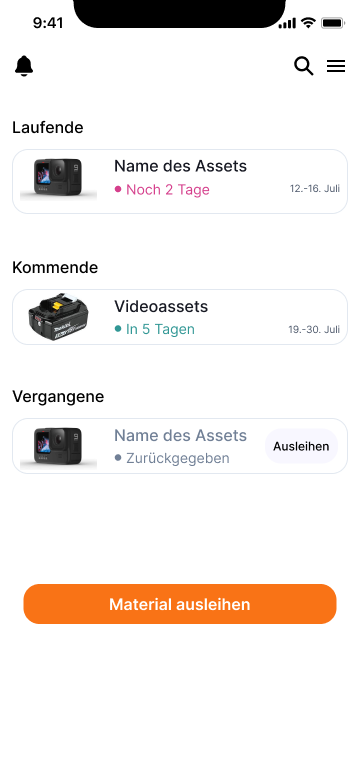
\includegraphics[scale=0.4]{Bilder/Prototyp/Start.png}\hspace{3em}
    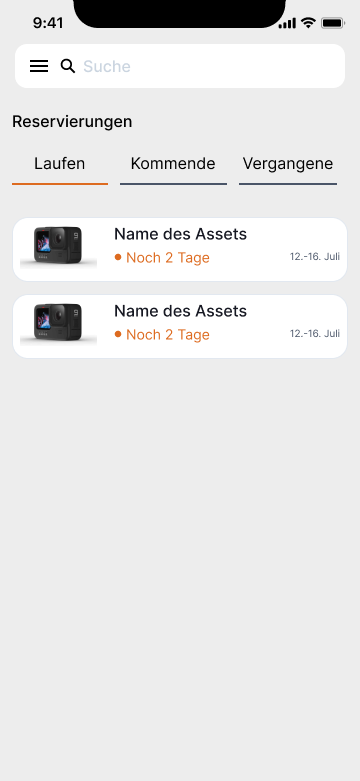
\includegraphics[scale=0.4]{Bilder/Prototyp/Neu/V2.png}
    \caption[Farbpalette]{Navigationsmüglichkeiten}
    \label{fig:home}
\end{figure}

\section{Navigation und Suchleiste}
In der Interface-Gestaltung gibt es verschiedene Möglichkeiten Navigation bereitzustellen. Für die
Anwendung wurde für den Mobilen Kontext eine Navigationsleiste am unteren Bildschirmrand und ein
Burgermenü oben Links oder Rechts in Erwägung gezogen. Für die Desktop-Navigation wurde zwischen
einer festen Navigationsleiste links und einer Leiste oben entscheiden. An Ende wurde sich für eine
Navigationsleiste auf der linken Seite entscheiden. Orientiert wurde sich hierbei an bekannten
Anwendungen mit ähnlichen Funktionen und dem Material Design \cite{google_material_2022}. Die
Umgangsweise mit diesen Gestaltungslösungen ist bereits bekannt und somit übertragbar (\textit{4
Beständigkeit und Standards} und \textit{6 Wiedererkennung statt Erinnerung} nach
\citeA{nielsen_enhancing_1994}). Daran Anknüpfend wurde sich für eine integrierte Suchleiste
entschieden, sodass Nutzende jederzeit die Möglichkeit haben, nach Assets zu suchen.

\begin{figure}[h]
    \centering
    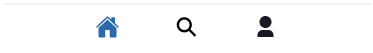
\includegraphics[scale=0.3]{Bilder/Prototyp/Property 1=Variant2.png}
    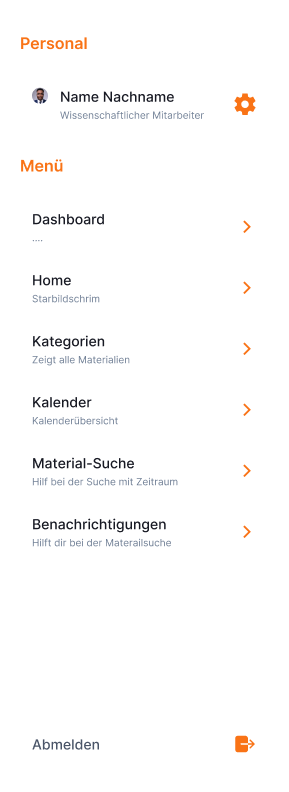
\includegraphics[scale=0.4]{Bilder/Prototyp/Menu.png}
    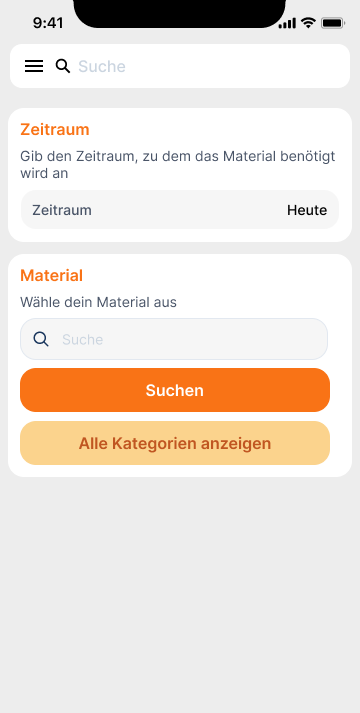
\includegraphics[scale=0.4]{Bilder/Prototyp/Neu/Suche V2.png}
    \caption[Farbpalette]{Navigationsmüglichkeiten}
    \label{fig:nav}
\end{figure}

\section{Kategorien und Suche}
Die Übersicht der Kategorien sind auch hier wieder an bekannten
Anwendungen mit ähnlichen Funktionen angelehnt (H4, H8). Dies führt unteren auch dazu, dass Fehler 
vermieden werden können (H9). 

Die Suche ist durch die Anwendung Airbnb\footnote{\url{https://www.airbnb.de/}} entstanden, das
viele Nutzende beim Reservieren von Dingen die Anwendung assoziieren (H2, H4). Die Suche sollte
durch das direkte einstellen eines Ausleihzeitraums Fehler vorbeugen und Verfügbarkeit anzeigen
(H5) (F-VA-6). \ref{fig:p1} zeigt die erste Version des High-Fidelity-Prototypen, bei welcher zum einen ein
Suchbutton fehlte und die Vorschläge der angezeigten Kategorien weniger genutzt wurden, sondern
direkt auf die Suche oder alle Anzeigen geklickt wurde, daher wurden diese Elemente entsprechenden 
angepasst (E1, E2, E4).

\begin{figure}[h]
    \centering
    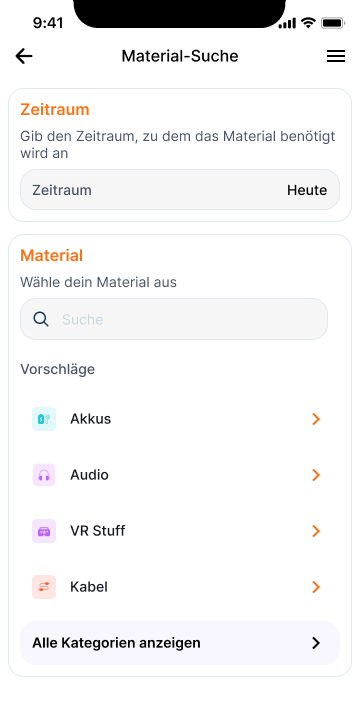
\includegraphics[scale=0.3]{Bilder/Prototyp/Suche.png}
    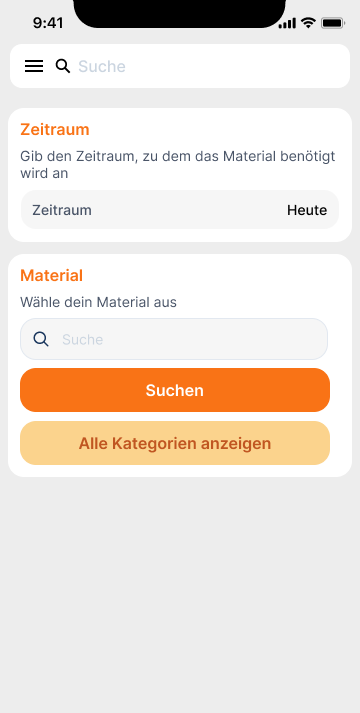
\includegraphics[scale=0.3]{Bilder/Prototyp/Neu/Suche V2.png}
    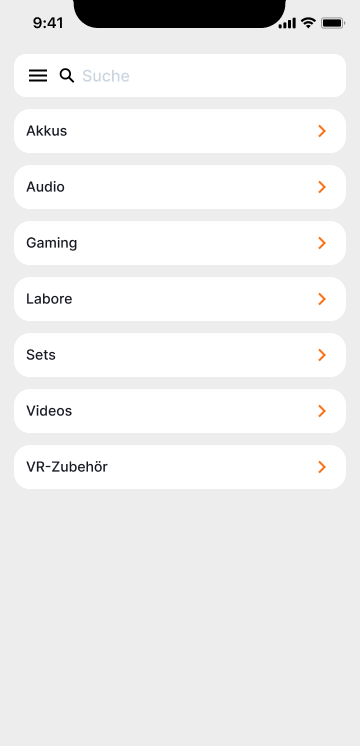
\includegraphics[scale=0.3]{Bilder/Prototyp/Neu/Kategorein 1.png}
    \label{fig:p1}
    \caption[Mockup: Kategorien, Assets, Assetdetails]{Kategorien (l), Assets (m), Assetdetails (r)}
\end{figure}

Kartenansicht einer Unterkategorie (H4, H8) (F-VA-3).

\begin{figure}[h]
    \centering
    \includegraphics[scale=0.3]{Bilder/Prototyp/Übersicht.png}
    \includegraphics[scale=0.3]{Bilder/Prototyp/Übersicht1.png}
    \label{fig:p4}
    \caption[Mockup: Kategorien, Assets, Assetdetails]{Kategorien (l), Assets (m), Assetdetails (r)}
\end{figure}


\section{Kalender}
Die Kalenderkomponente wurde lediglich als Skizze veranschaulicht. In den High-Fidelity-Prototyp
wurde sich bereits an der Komponenten V-Calendar\footnote{\url{https://vcalendar.io/layouts.html}}
orientiert, welche die wichtigsten Funktionen mitbrachte und so die Realisierung erleichtert.

Bei dem Kalender war es unteranderem wichtig, dass Wochenenden ausgeblendet werden können, da zu
diesen Zeitpunkten keine Ausleihe möglich ist, außerdem sollten vergangene Tage nicht auswählbar
sein. Weitere Punkte wurden auch hier wieder von der Anwendung Airbnb angeschaut (H1,4,7,8) (E2-4)
(F-VA-3). Für Verleihende ist eine Todolistenansicht, was den Tag über ansteht wichtig
gewesen (F-V-4). \ref{fig:kalender}

\begin{figure}[h]
    \centering
    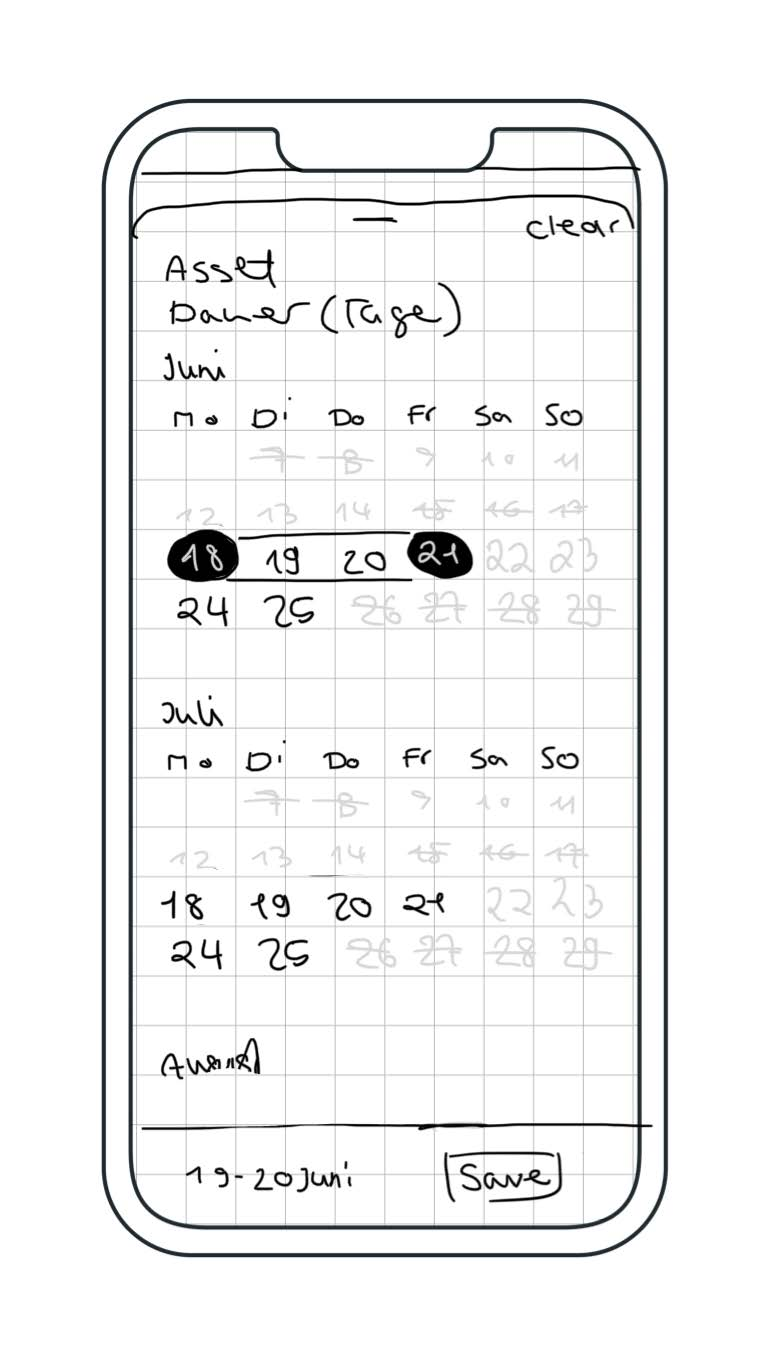
\includegraphics[scale=0.37]{Bilder/Mockups/Kalender.jpg}
    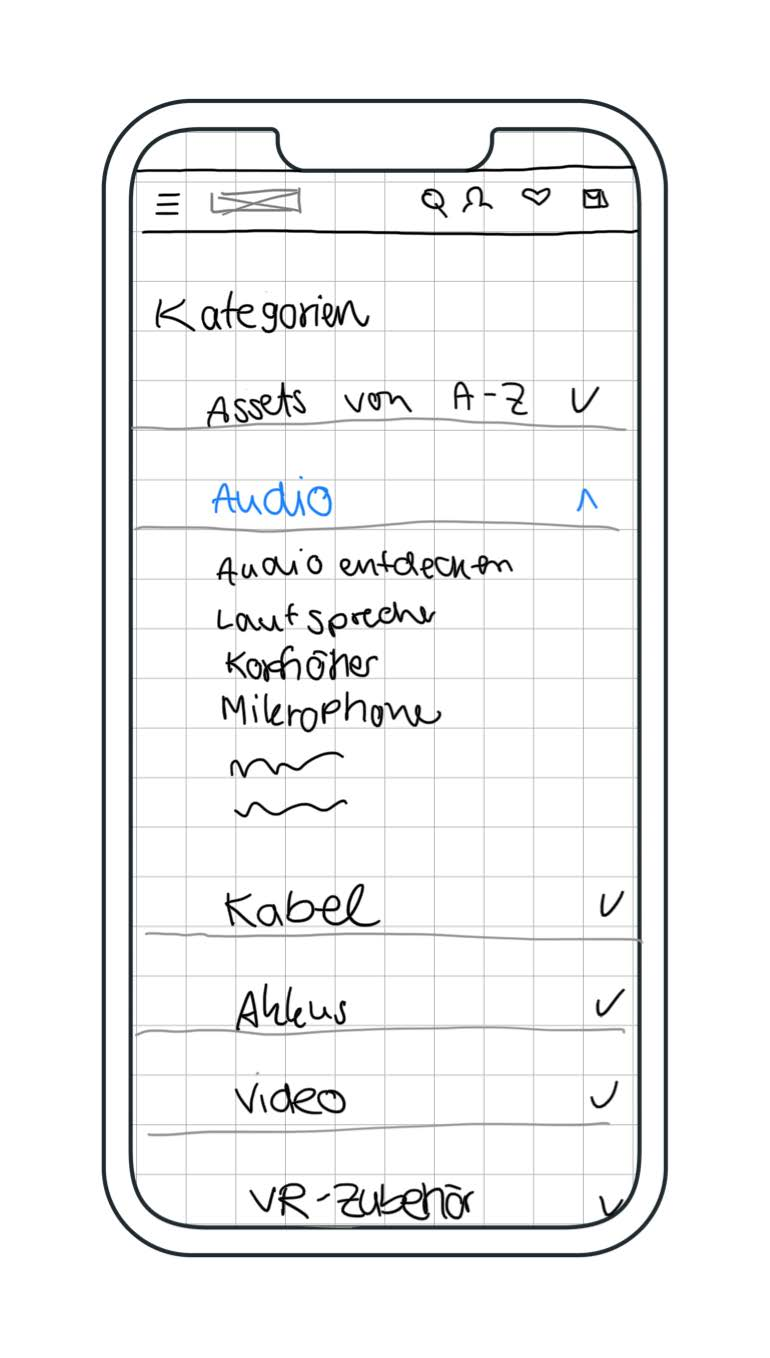
\includegraphics[scale=0.37]{Bilder/Mockups/Kategorien.jpg}
    \label{fig:kalender}
\caption[Kalenderkomponente]{Kalender (l), Navigation (r)}
\end{figure}



\section{Asset-Detailansicht und Reservierungen}
Die Ansicht der einzelnen Assets sollte insbesondere Assetverfügbarkeit, Funktionalitäten sowie
Verleihende enthalten (F-VA-3, F-VA-4, F-VA-8). \ref{fig:p3} zeigt ..

Es ergab sich, dass eine Beschreibung des Artikels erstmal nicht von Bedeutung ist (E6).

Die Reservierung eines Assets ... der Zeitraum einzelnt unnötig, daher geändert (E5). Wording auch
hier überarbeitet (F-A-2) 

Warum Ausleihzeitraum separat zu Abholung und Rückgabe -> Impliziert das bereits

\begin{figure}[h]
    \centering
    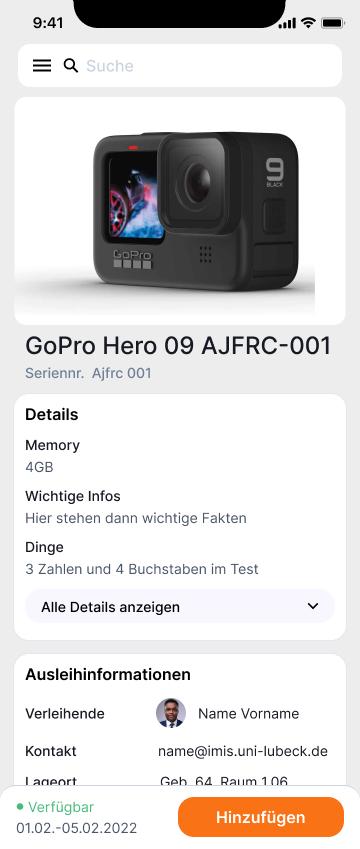
\includegraphics[scale=0.3]{Bilder/Prototyp/Neu/Datailansicht-1.png}
    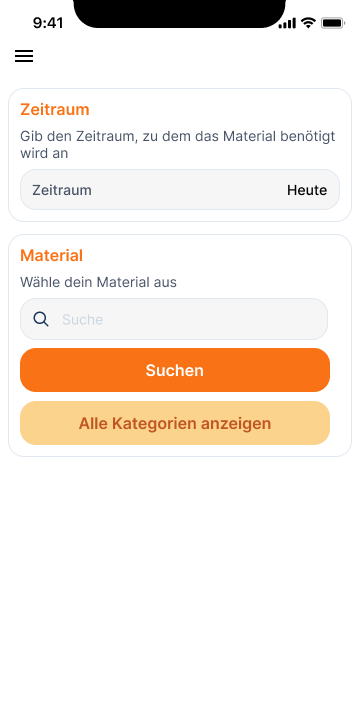
\includegraphics[scale=0.3]{Bilder/Prototyp/Neu/Suche.png}
    \includegraphics[scale=0.3]{Bilder/Prototyp/Reservierung abschließen 3.png}
    \label{fig:p3}
    \caption[Mockup: Kategorien, Assets, Assetdetails]{Kategorien (l), Assets (m), Assetdetails (r)}
\end{figure}




